\documentclass{article}

% Packages
\usepackage{amsmath}    
\usepackage{graphicx}   
\usepackage{float}      
\usepackage{booktabs}   
\usepackage{neurips_2024}
\usepackage[utf8]{inputenc}
\usepackage[T1]{fontenc}
\usepackage{hyperref}
\usepackage{url}
\usepackage{amsfonts}
\usepackage{nicefrac}
\usepackage{microtype}
\usepackage{xcolor}

\begin{document}

\title{Support Vector Machines for Credit Default Prediction}


\maketitle

\begin{abstract}
This project presents an analysis of support vector machines (SVMs) applied to the UCI Default of Credit Card Clients dataset. 
The study investigates how different kernal functions and optimization techniques influence classification performance. 
Support Vector Machine models using linear, radial basis function (RBF), polynomial, and sigmoid kernels are evaluted. 
A grid search is conducted for hyperparameter optimization, and PCA is utilized to visualize decision boundaries. 
Performance metrics, including accuracy, precision, recall, F1 score, and runtime are used to evaluate the results, 
highlighting the effectiveness of SVM's in binary classification tasks involving tabular data.
\end{abstract}

\section{Introduction}
Support vector machines (SVMs) are a widely used supervised machine learning approach, recognized for their strong performance 
in diverse classification tasks. This project explores the application of Support Vector Machines to the UCI Default of Credit Card 
Clients dataset, focusing on the role of kernal functions and optimization techniques in shaping model performance. Additionally, 
hyperparameter tuning is investigated as a means of improving both effiency and accuracy. To improve interpretability, Principal Component Analysis (PCA) 
is used to visualize the decision boundries. The main goal is to evaluate the effectiveness of SVM's for predicting credit card default and to analyze the 
computational trade-offs associated with various kernel functions and optimization strategies. Results are evaluated using accuracy, recall, precision, and the F1-score.



\section{Dataset}

The UCI Default of Credit Card Clients dataset is a multivariate dataset containing data from 30,000 credit card holders in Taiwan. 
It is primarily designed for binary classification tasks, specifically predicting whether a client would default on their next months payment. 
The dataset includes 23 features, which consist of demographic variables such as age, sex, education, and marital status, along with financial metrics like credit limits, 
historical bill statements, and repayment amounts. The target variable is binary, indicating whether a client defaulted (1) or did not default (0) on their credit card payment. 

The dataset includes a mix of categorical and numerical variables. Important variables include repayment statuses (\texttt{PAY\_0} to \texttt{PAY\_6}), 
historical bill amounts (\texttt{BILL\_AMT1} through \texttt{BILL\_AMT6}), and historical repayment amounts (\texttt{PAY\_AMT1} to \texttt{PAY\_AMT6}). 
Additionally, demographic variables such as \texttt{SEX}, \texttt{EDUCATION}, and \texttt{MARRIAGE} provide insights into customer profiles. Table~\ref{variables_table} 
summarizes the key features in the dataset.

\begin{table}[H]
\centering
\caption{Summary of Key Features in the Dataset}
\label{variables_table}
\begin{tabular}{@{}lcll@{}}
\toprule
\textbf{Variable Name} & \textbf{Type} & \textbf{Description}                  & \textbf{Units}       \\ \midrule
SEX                    & Categorical   & Gender                                & 1 = Male, 2 = Female \\ 
EDUCATION              & Categorical   & Education level                       & 1 = Graduate, etc.   \\ 
MARRIAGE               & Categorical   & Marital status                        & 1 = Married, etc.    \\ 
BILL\_AMT1-6           & Numerical     & Monthly bill amounts (6 months)       & NT Dollars           \\ 
PAY\_AMT1-6            & Numerical     & Historical repayment amounts (6 months) & NT Dollars         \\ 
PAY\_0-6               & Categorical   & Repayment status (-2: advance payment) & Discrete values      \\ 
DEFAULT (Target)       & Binary        & Default status for the next month     & 0 = No, 1 = Yes      \\ \bottomrule
\end{tabular}
\end{table}

To prepare the dataset for modeling, several preprocessing steps were applied. Variables like \texttt{SEX}, \texttt{EDUCATION}, \texttt{MARRIAGE}, 
and repayment statuses (\texttt{PAY\_0} to \texttt{PAY\_6}) were categorical. Since SVMs require numerical input, these categorical variables 
were transformed into one-hot encoded binary variables. This ensured that each category was treated as an independent feature, avoiding any implicit ordinal assumptions. 
Additionally, the dataset exhibited significant class imbalance, as most clients did not default on their payments. To address this, the majority class (non-default clients) 
was downsampled to create a balanced dataset. This ensured the model learned patterns equally well from defaulting and non-defaulting clients.

Another essential step was standardizing numerical features like bill amounts and repayment amounts. These features had varying scales, with some measured in monetary units and others being categorical. 
Without standardization, features with larger magnitudes could disproportionately impact the model. Thus, all continuous features were scaled to have a mean of zero and a standard deviation of one, 
ensuring fair contribution from all variables.

The preprocessing steps of one-hot encoding, downsampling, and standardization were essential to making the dataset compatible with SVMs and producing reliable predictions. 
These transformations addressed challenges posed by mixed feature types, class imbalance, and variable scaling, ultimately improving the efficiency and accuracy of the machine learning models used in this study.


\section{Methodology}
The Support Vector Machine (SVM) algorithm aims to find an optimal hyperplane that maximizes the margin between two classes while minimizing classification errors. For a training dataset with n points $\{(\mathbf{x}_i, y_i)\}_{i=1}^n$ where $\mathbf{x}_i \in \mathbb{R}^d$ and $y_i \in \{-1, 1\}$, the primal optimization problem is formulated as:

\[
\min_{\mathbf{w}, b, \xi} \frac{1}{2} \|\mathbf{w}\|^2 + C \sum_{i=1}^n \xi_i
\]

subject to the constraints:
\[
y_i(\mathbf{w}^\top\mathbf{x}_i + b) \geq 1 - \xi_i, \quad \xi_i \geq 0, \quad i = 1,\ldots,n
\]

where $\mathbf{w}$ is the normal vector to the hyperplane, $b$ is the bias term, $\xi_i$ are slack variables allowing for soft margin violations, and $C$ is the regularization parameter controlling the trade-off between margin maximization and error minimization.

The dual formulation of this optimization problem, derived using Lagrange multipliers, is:

\[
\max_{\boldsymbol{\alpha}} \sum_{i=1}^n \alpha_i - \frac{1}{2}\sum_{i=1}^n\sum_{j=1}^n \alpha_i\alpha_j y_i y_j \mathbf{x}_i^\top\mathbf{x}_j
\]

subject to:
\[
0 \leq \alpha_i \leq C, \quad i = 1,\ldots,n \quad \text{and} \quad \sum_{i=1}^n \alpha_i y_i = 0
\]

To handle nonlinear classification problems, kernel functions $K(\mathbf{x}_i, \mathbf{x}_j)$ are introduced to implicitly map the input features into a higher-dimensional space. The kernel trick transforms the dual optimization problem to:

\[
\max_{\boldsymbol{\alpha}} \sum_{i=1}^n \alpha_i - \frac{1}{2}\sum_{i=1}^n\sum_{j=1}^n \alpha_i\alpha_j y_i y_j K(\mathbf{x}_i, \mathbf{x}_j)
\]

In this project, four kernel functions were evaluated:
\begin{enumerate}
    \item Linear: $K(\mathbf{x}_i, \mathbf{x}_j) = \mathbf{x}_i^\top\mathbf{x}_j$
    \item Polynomial: $K(\mathbf{x}_i, \mathbf{x}_j) = (\gamma\mathbf{x}_i^\top\mathbf{x}_j + r)^d$
    \item RBF (Gaussian): $K(\mathbf{x}_i, \mathbf{x}_j) = \exp(-\gamma\|\mathbf{x}_i - \mathbf{x}_j\|^2)$
    \item Sigmoid: $K(\mathbf{x}_i, \mathbf{x}_j) = \tanh(\gamma\mathbf{x}_i^\top\mathbf{x}_j + r)$
\end{enumerate}

The decision function for classifying new points becomes:

\[
f(\mathbf{x}) = \text{sign}\left(\sum_{i=1}^n \alpha_i y_i K(\mathbf{x}_i, \mathbf{x}) + b\right)
\]

Grid search cross-validation was employed to optimize the hyperparameters $C$ and $\gamma$ for each kernel. The search space included:
\begin{itemize}
    \item $C \in \{0.1, 1, 10, 100\}$
    \item $\gamma \in \{0.001, 0.01, 0.1, 1\}$
\end{itemize}

To facilitate visualization and interpretation, Principal Component Analysis (PCA) was applied to reduce the feature space to two dimensions. Given the centered data matrix $\mathbf{X} \in \mathbb{R}^{n \times d}$, where $n$ is the number of samples and $d$ is the number of features, PCA first computes the covariance matrix:

\[
\mathbf{\Sigma} = \frac{1}{n}\mathbf{X}^\top\mathbf{X}
\]

PCA then performs eigendecomposition of the covariance matrix:

\[
\mathbf{\Sigma} = \mathbf{V}\boldsymbol{\Lambda}\mathbf{V}^\top
\]

where $\mathbf{V} \in \mathbb{R}^{d \times d}$ contains the eigenvectors as columns (sorted by decreasing eigenvalues) and $\boldsymbol{\Lambda} = \text{diag}(\lambda_1, \ldots, \lambda_d)$ contains the corresponding eigenvalues. The transformed features are obtained by projecting the data onto the first two principal components:

\[
\mathbf{X}_{\text{transformed}} = \mathbf{X}\mathbf{V}_{1:2}
\]

where $\mathbf{V}_{1:2} \in \mathbb{R}^{d \times 2}$ contains the first two eigenvectors. This projection preserves the maximum possible variance in the data while reducing dimensionality to facilitate visualization of the decision boundaries.


\section{Results}
The comparative analysis of kernel functions yielded results, summarized in Table~\ref{kernel-results}. The RBF kernel outperformed other kernels, achieving the highest accuracy (68.75\%) and F1-score (0.65). 
The scree plot in Figure~\ref{fig:scree-plot} highlights the explained variance by the principal components, providing insights into the dimensionality reduction process.

\begin{figure}[H]
    \centering
    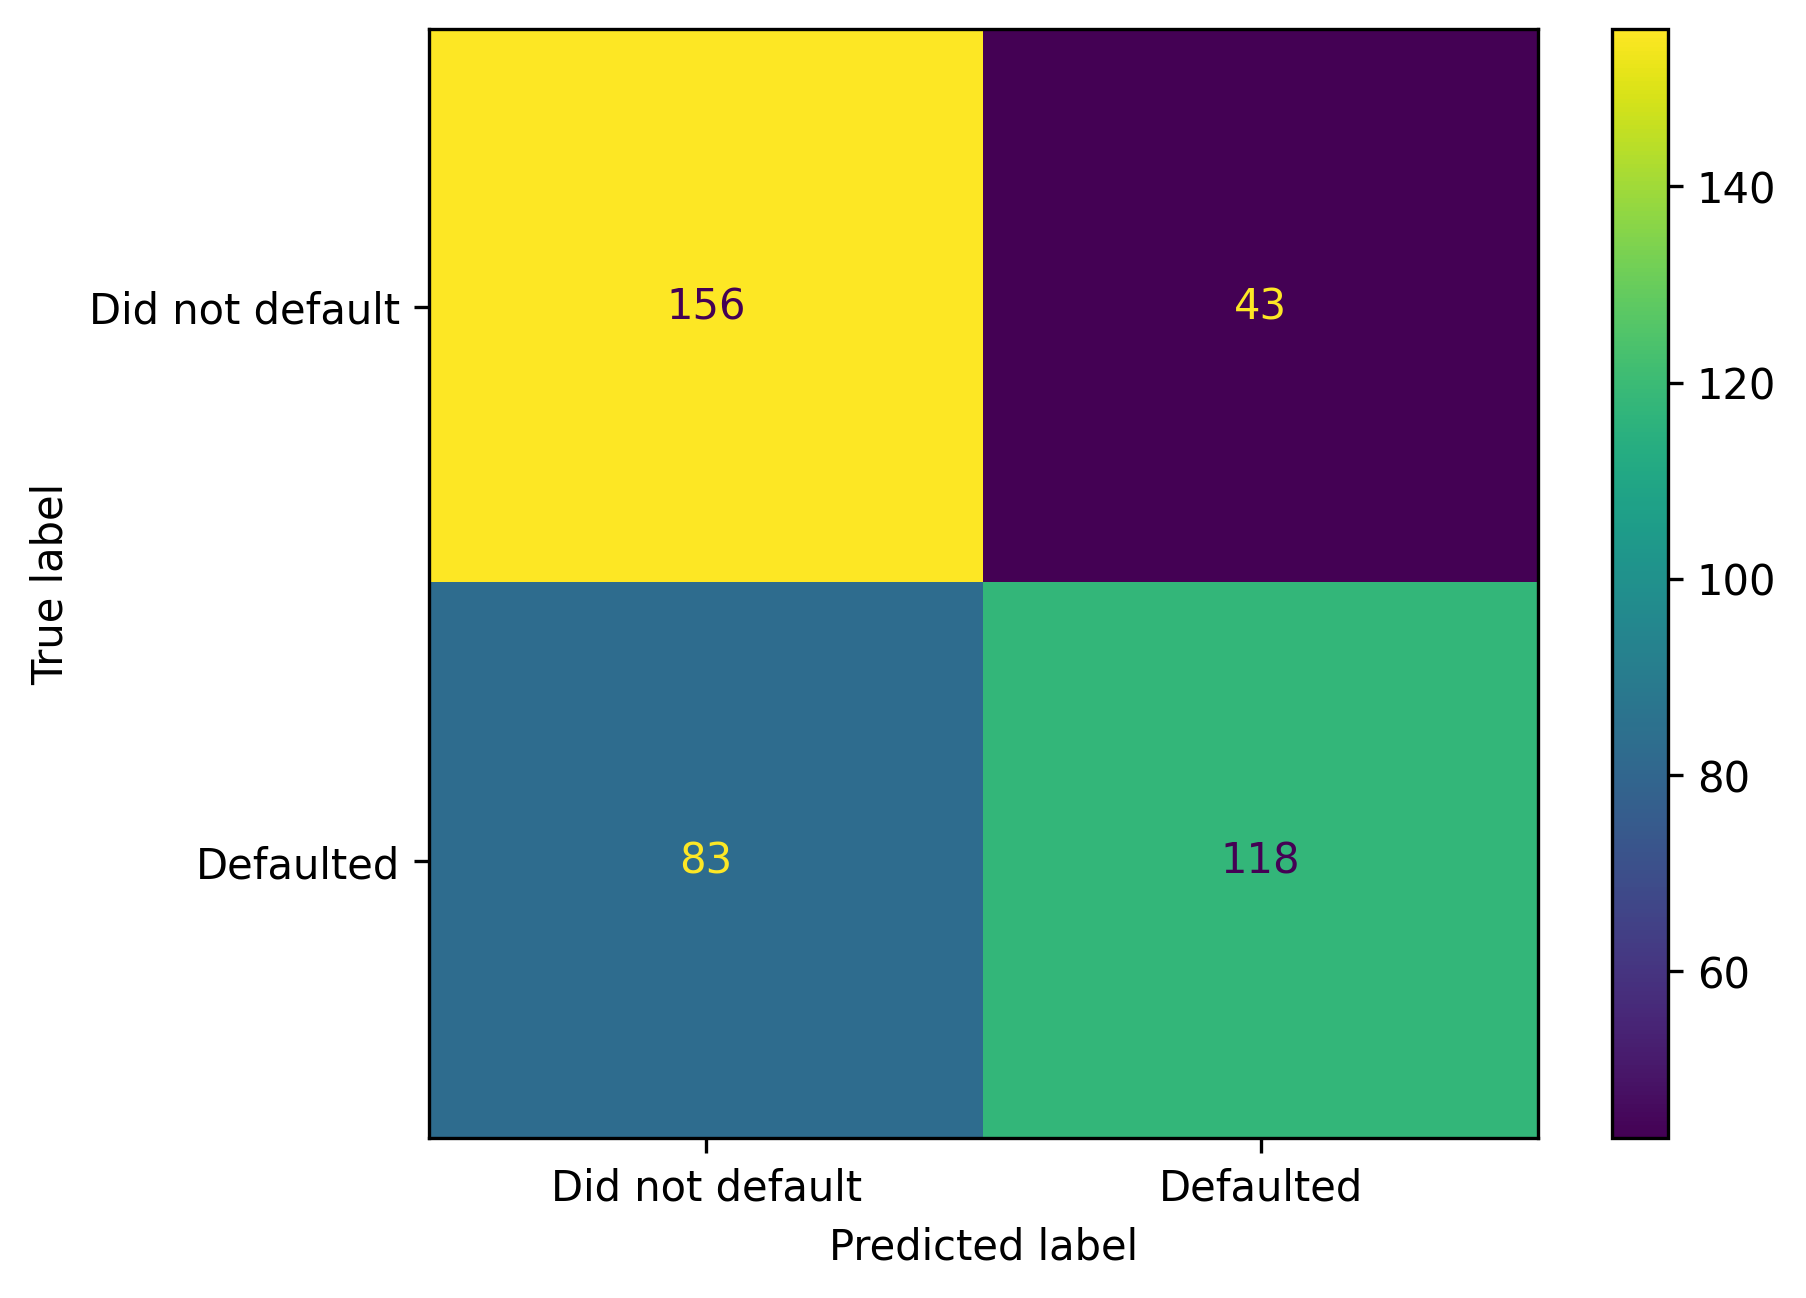
\includegraphics[width=0.7\textwidth]{../figures/confusion_matrix_pre_gridSearch.png}
    \caption{Confusion Matrix Before Grid Search.}
    \label{fig:confusion-pre-grid}
\end{figure}

\begin{figure}[H]
    \centering
    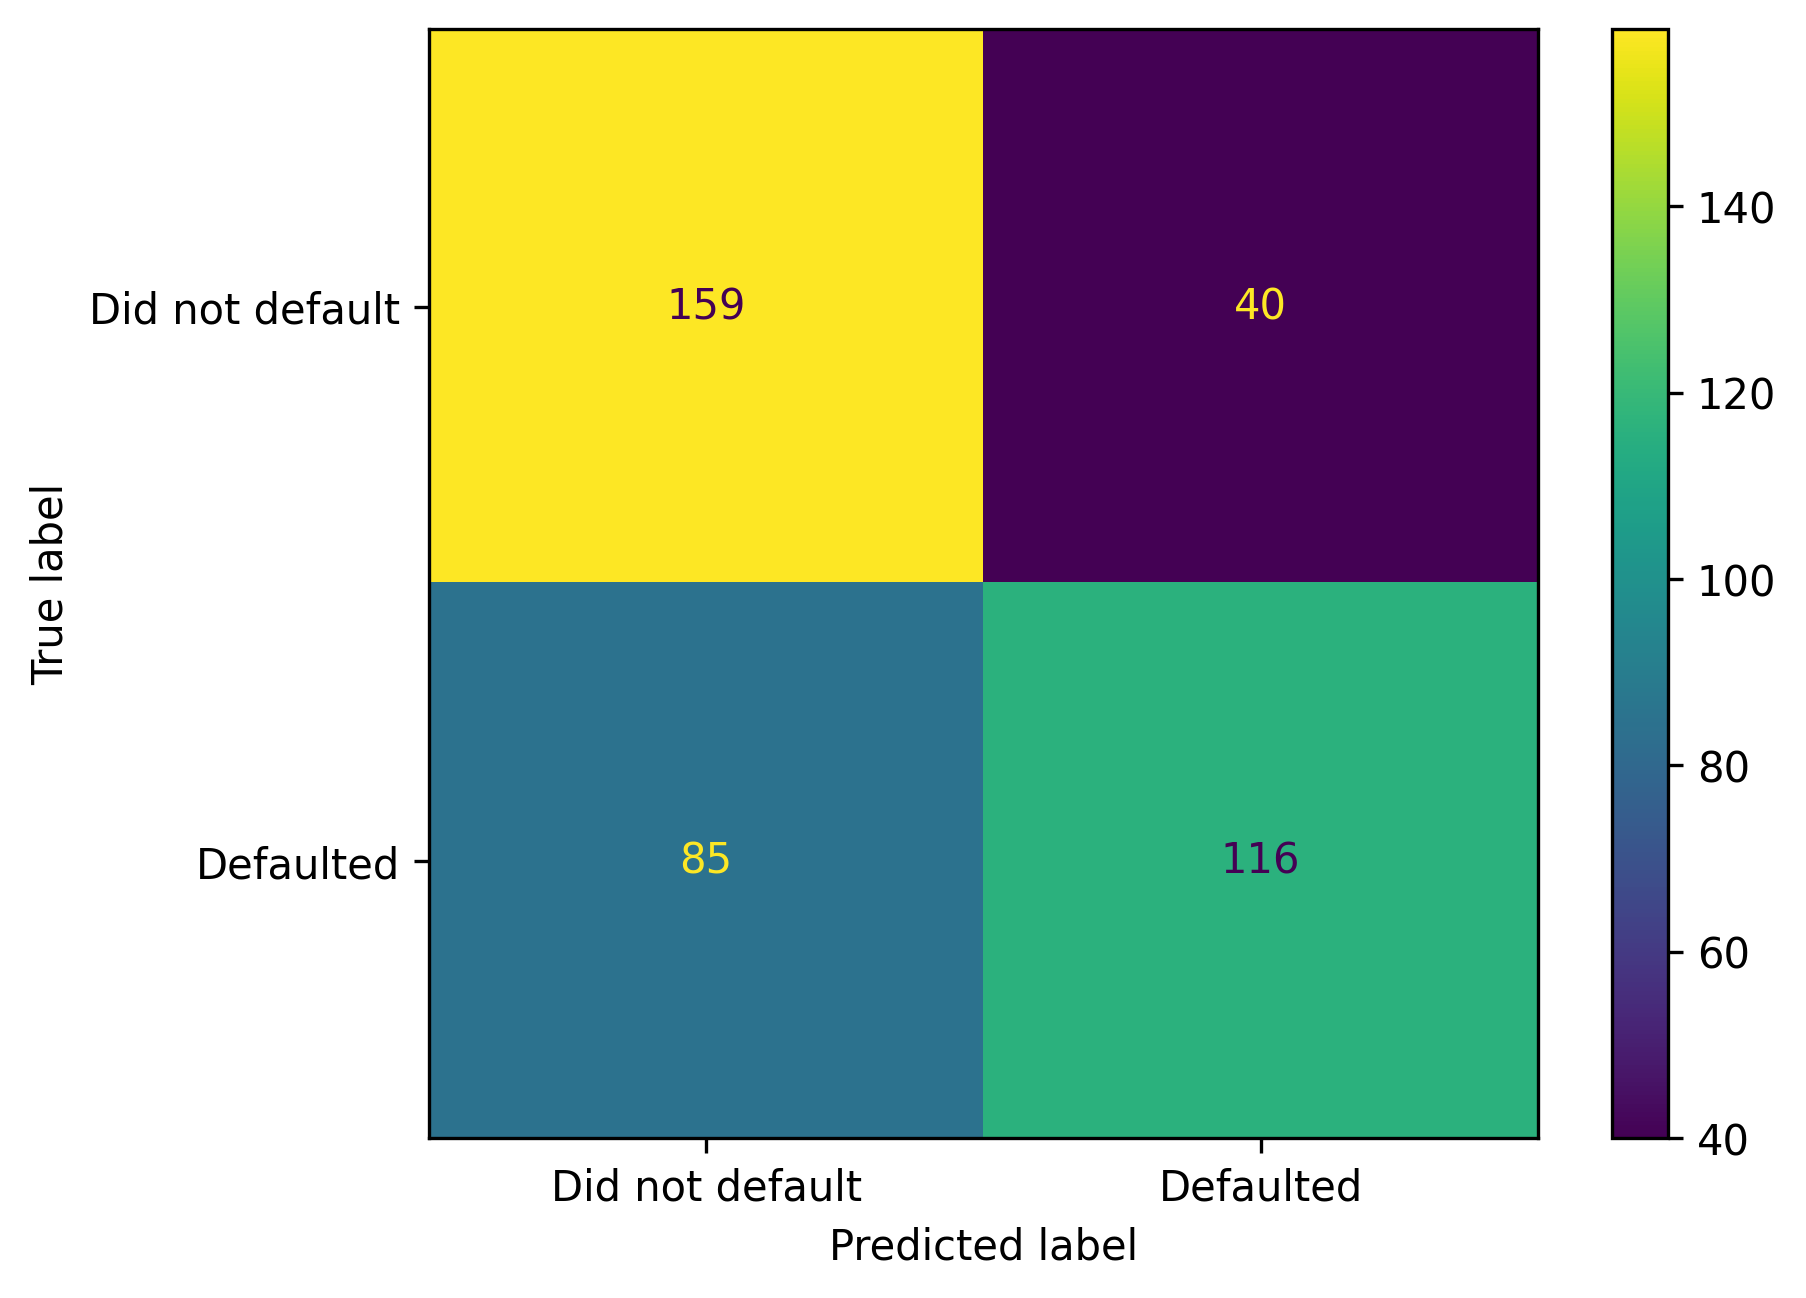
\includegraphics[width=0.7\textwidth]{../figures/confusion_matrix_post_gridSearch.png}
    \caption{Confusion Matrix After Grid Search.}
    \label{fig:confusion-post-grid}
\end{figure}

\begin{table}[H]
\centering
\caption{Kernel Comparison Results}
\label{kernel-results}
\begin{tabular}{@{}lcccccc@{}}
\toprule
\textbf{Kernel} & \textbf{Accuracy} & \textbf{Precision} & \textbf{Recall} & \textbf{F1-Score} & \textbf{Runtime (s)} & \textbf{Best Hyperparameters (C, $\gamma$)} \\ \midrule
Linear          & 0.6525            & 0.7095             & 0.5224          & 0.6017            & 0.2457              & (1, Scale)                                    \\ 
Polynomial      & 0.6700            & 0.7226             & 0.5572          & 0.6292            & 0.0629              & (10, 0.01)                                   \\ 
RBF             & 0.6875            & 0.7436             & 0.5771          & 0.6499            & 0.0634              & (1, 0.01)                                    \\ 
Sigmoid         & 0.6450            & 0.7007             & 0.5124          & 0.5920            & 0.0891              & (100, 0.001)                                 \\ \bottomrule
\end{tabular}
\end{table}

\begin{figure}[H]
    \centering
    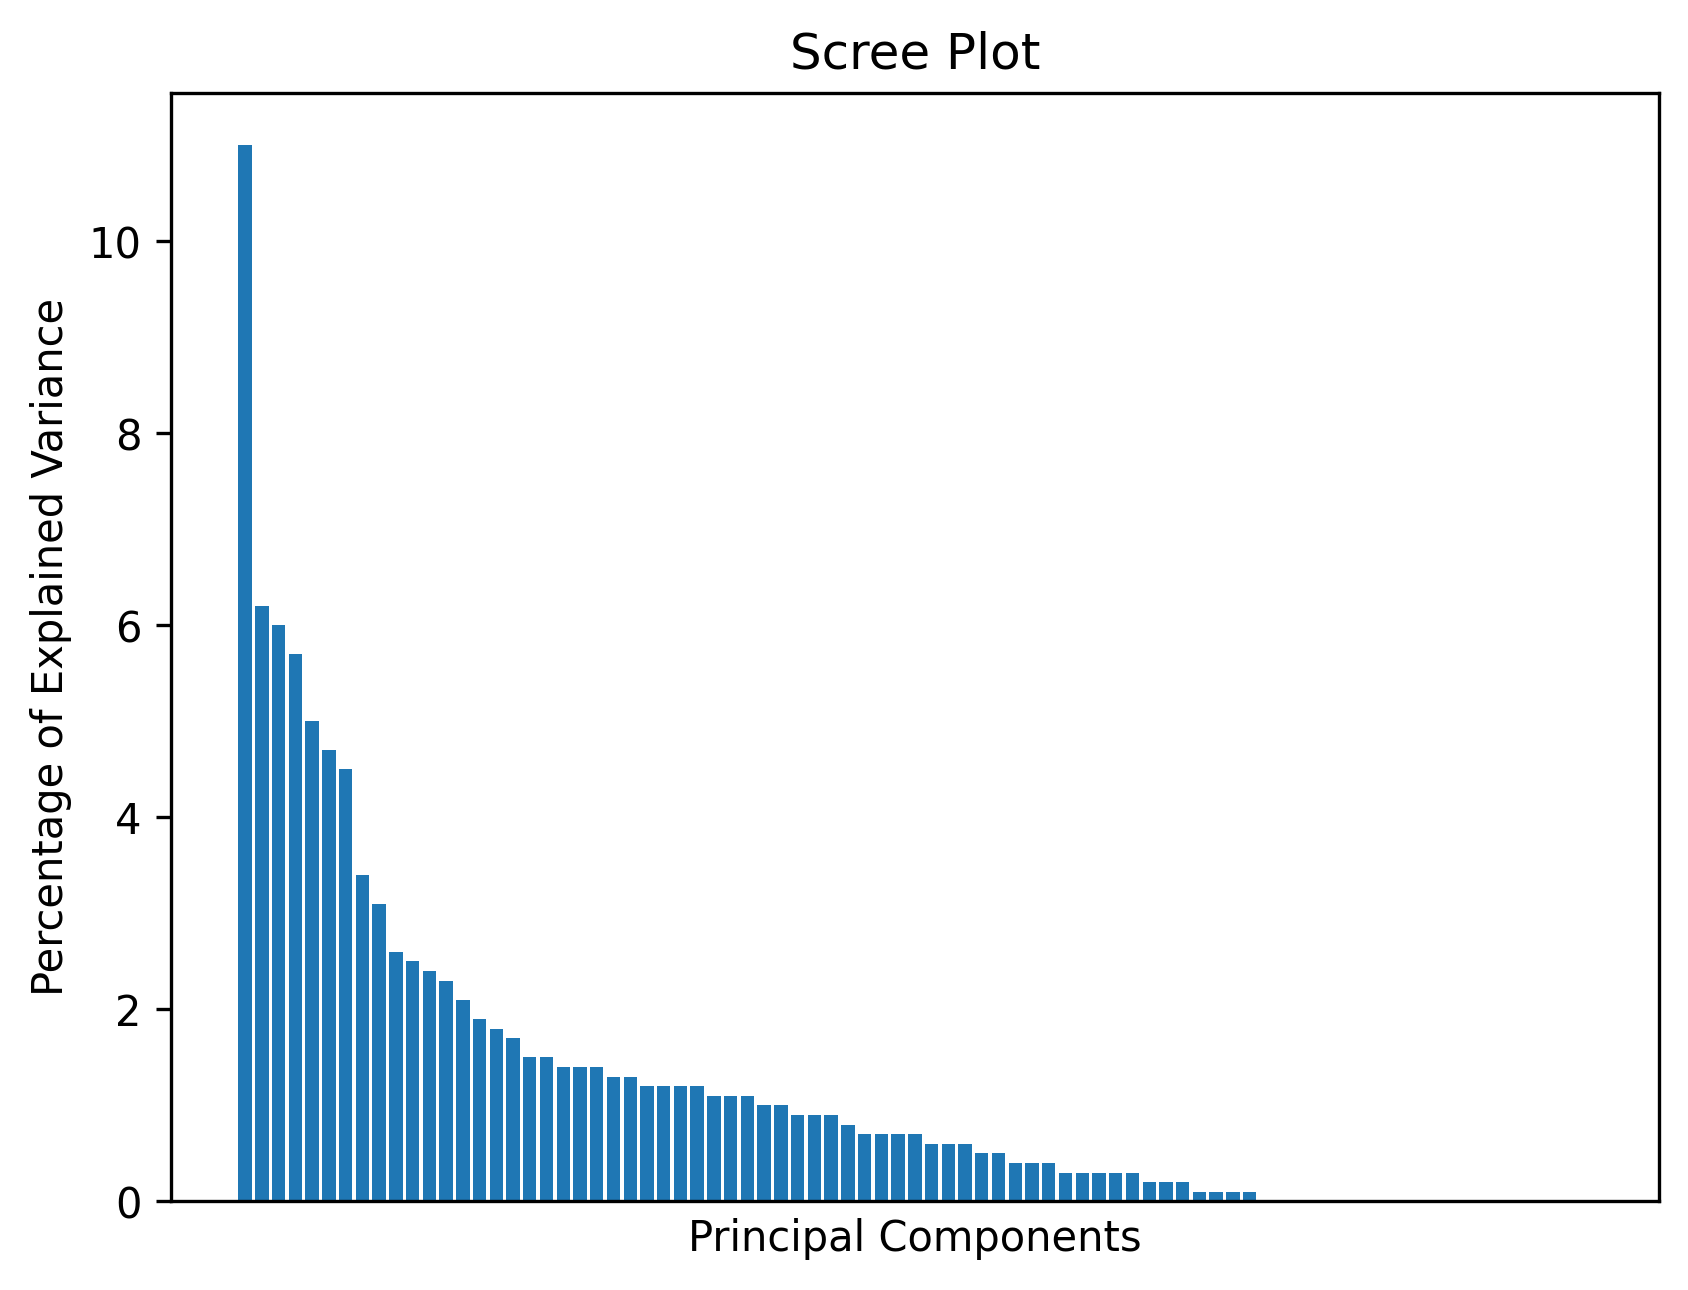
\includegraphics[width=0.7\textwidth]{../figures/scree_plot.png}
    \caption{Scree Plot Showing Percentage of Explained Variance.}
    \label{fig:scree-plot}
\end{figure}

\begin{figure}[H]
    \centering
    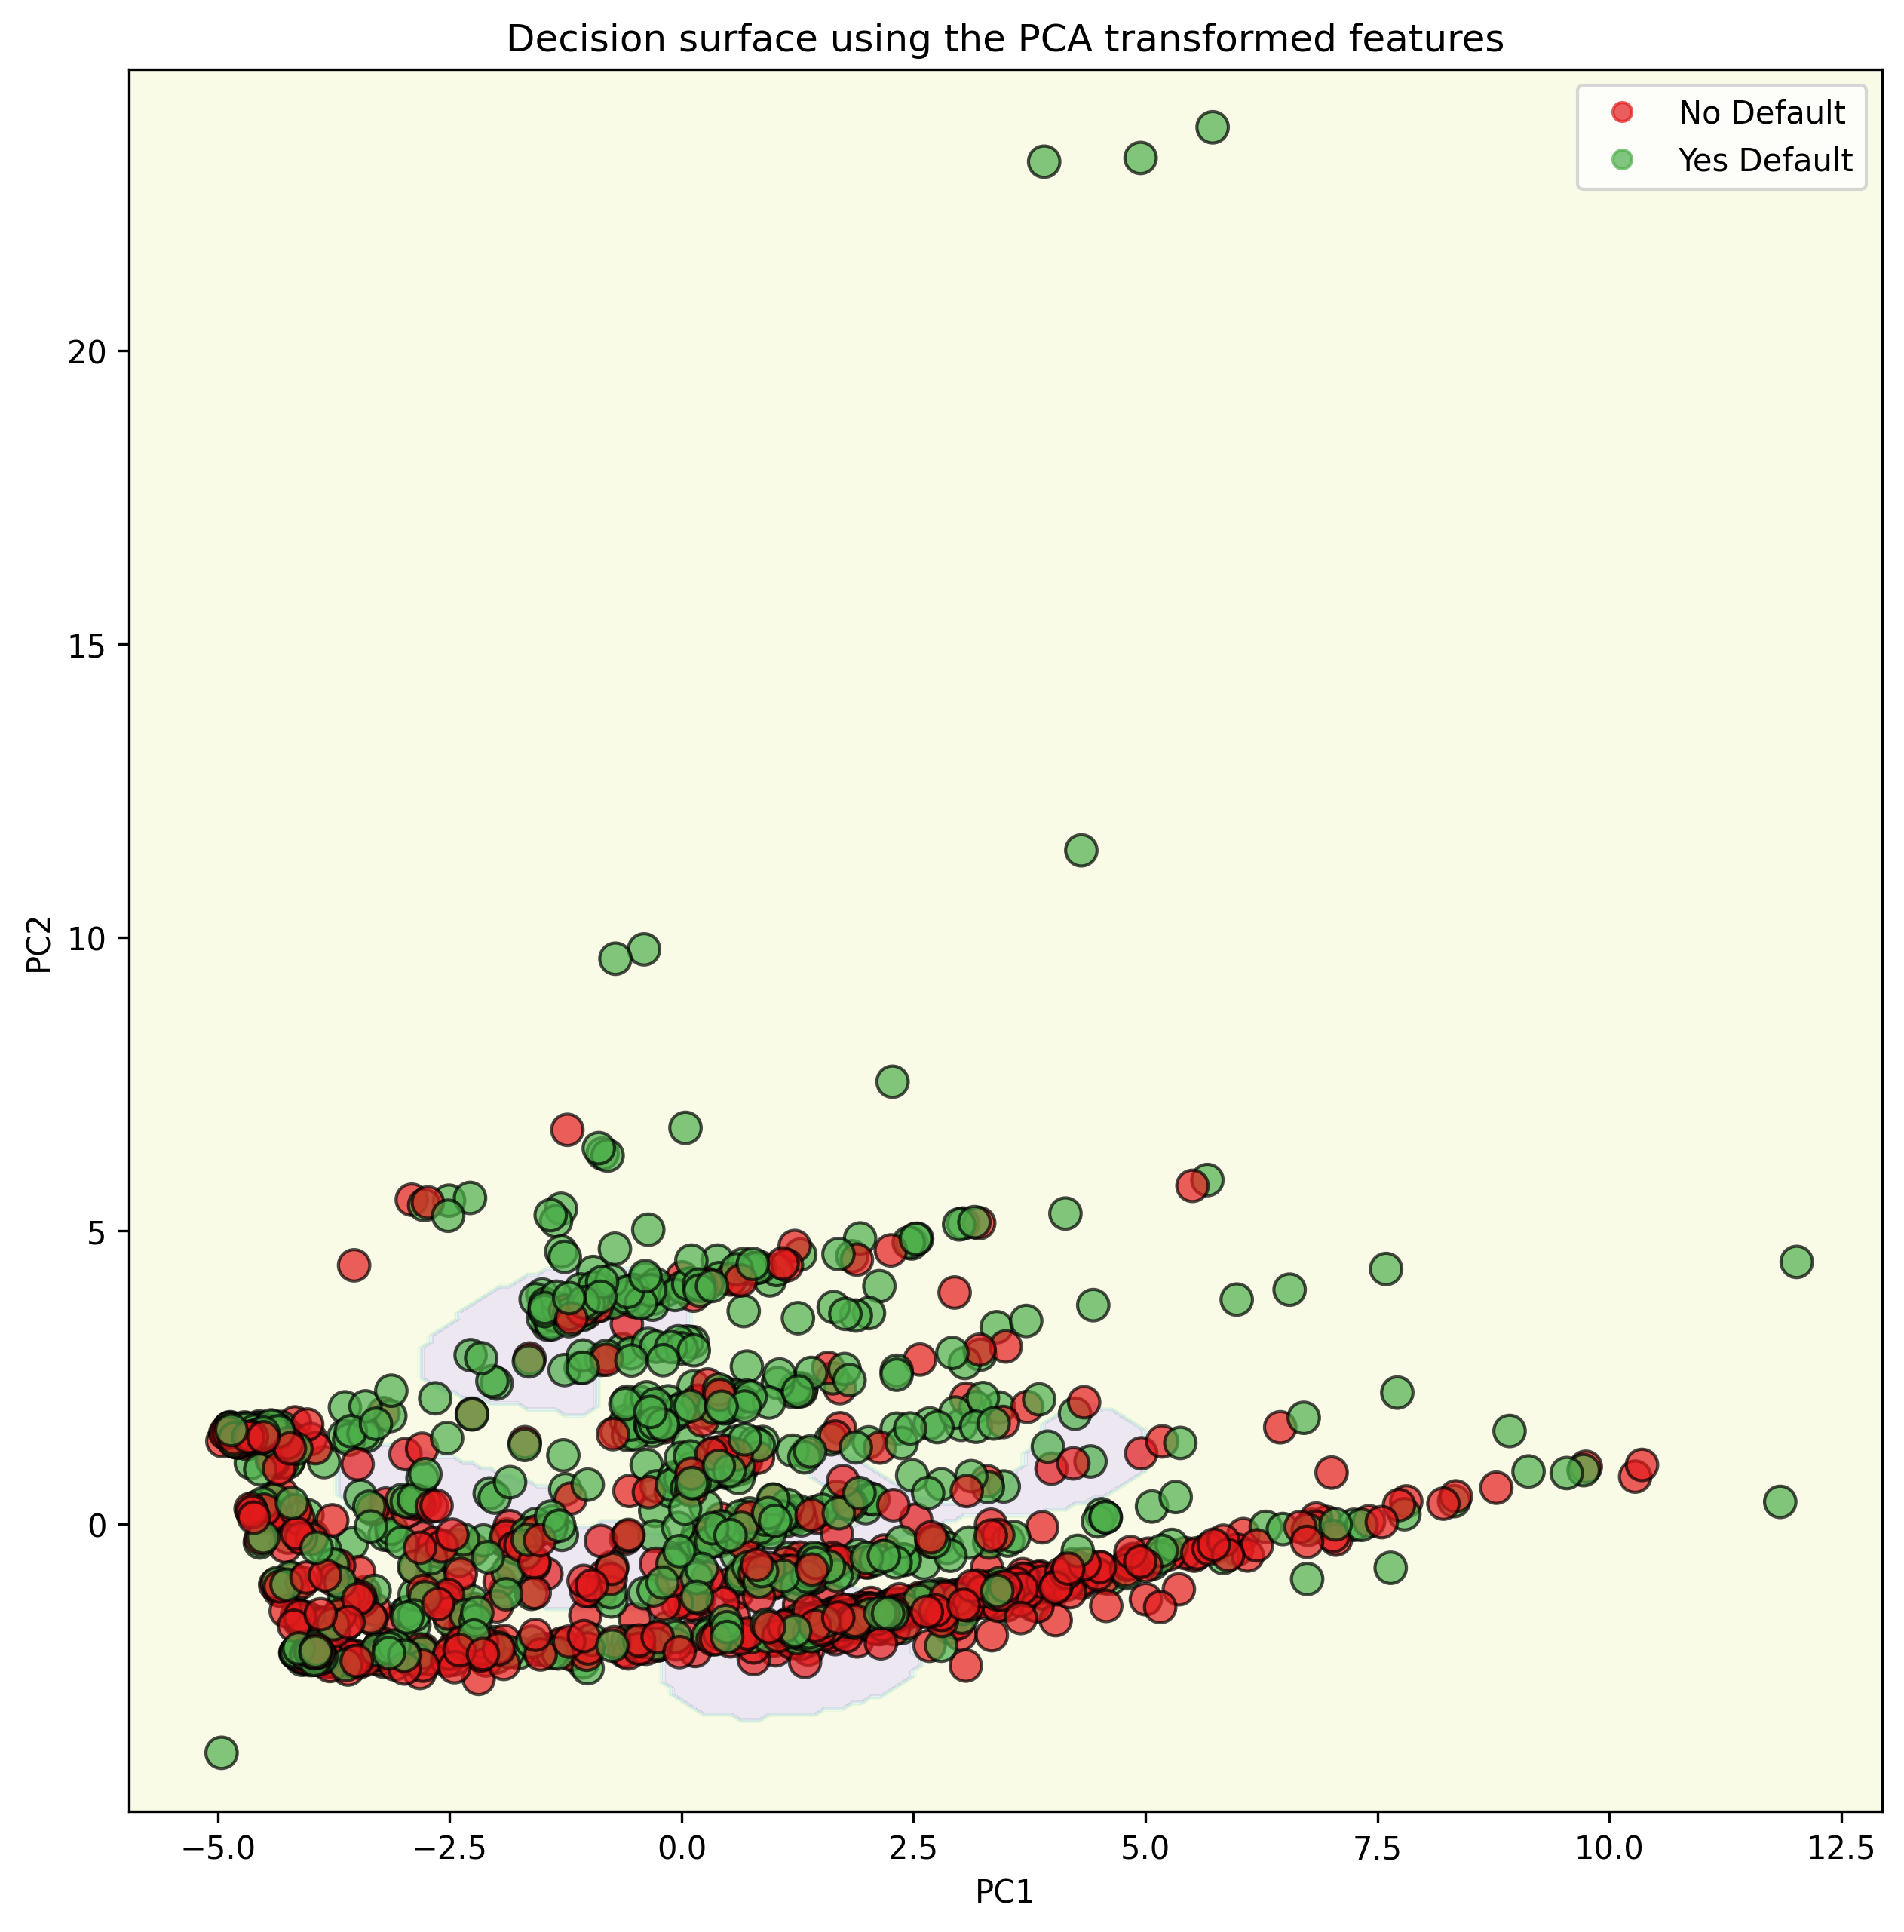
\includegraphics[width=0.7\textwidth]{../figures/decision_surface_pca.png}
    \caption{Decision Surface Using PCA Transformed Features.}
    \label{fig:decision-surface}
\end{figure}

\section{Discussion}

The results highlight the importance of kernel selection in SVMs for binary classification tasks. Among the evaluated kernels, the radial basis function (RBF) kernel stood out as the 
best performing option, achieving an accuracy of 68.75\%. This performance underscores the RBF kernel's strength in mapping data into higher-dimensional spaces, allowing it to capture nonlinear decision boundaries. 
However, the achieved accuracy remains relatively modest, raising questions about whether SVMs are the most suitable choice for this dataset. While the polynomial kernel showed comparable performance with an accuracy of 67.00\%, 
its sensitivity to parameter tuning limited its robustness. In contrast, the linear kernel underperformed, achieving an accuracy of only 65.25\%, which likely results from its inability to handle the nonlinear structure in the data. 
The sigmoid kernel, with its more complex parameterization, struggled to converge effectively and resulted in the lowest accuracy of 64.50\%.

The relatively low accuracy across all kernels suggests that SVMs, while effective in many applications, may not be the optimal model for this task. The imbalanced and high-dimensional nature of the dataset likely contributed to these results. 
Although hyperparameter tuning through grid search improved the models as seen in the enhanced confusion matrix after optimization (Figure~\ref{fig:confusion-post-grid})—the improvements were incremental and insufficient to achieve significant gains in accuracy. 
This points to challenges inherent in the dataset, such as overlapping class distributions and complex feature relationships, that SVMs alone might not effectively address.

The PCA visualization of the decision boundary (Figure~\ref{fig:decision-surface}) offered insights into the separability of the classes. However, the limited explained variance from the first two principal components (Figure~\ref{fig:scree-plot}) 
suggests that most of the dataset's complexity lies in higher dimensions. This indicates a limitation of PCA for interpretability and hints that other dimensionality reduction techniques could provide more nuanced insights into the data's structure.

\section{Conclusion}

This project demonstrates the limitations of SVMs for predicting credit card default, with even the best performing RBF kernel achieving only 68.75\% accuracy. While the findings emphasize the importance of kernel selection, none of the tested kernels 
achieved performance levels that would be satisfactory for real-world application. Although hyperparameter tuning via grid search led to minor improvements, the gains were not substantial enough to overcome the inherent limitations of SVMs for this specific problem.

The suboptimal performance across all kernel types, ranging from 64.50\% to 68.75\% accuracy, indicates that SVMs may not be well-suited for credit card default prediction on this dataset. The complex, high-dimensional nature of the data, 
combined with likely class overlap, presents significant challenges that SVMs struggle to address. Future work should focus on exploring more advanced machine learning techniques, such as ensemble methods or deep learning models, which could be better equipped to 
handle the complexities of credit default prediction. Additionally, investigating alternative feature engineering techniques and addressing the dataset's underlying issues may yield greater improvements than further optimizing SVM models.


\section*{References}
\begin{itemize}
    \item Agarwal, A. (2023). Everything About SVM Classification: Above and Beyond. \textit{Towards Data Science}. Available at \url{https://towardsdatascience.com/everything-about-svm-classification-above-and-beyond-cc665bfd993e}.
    \item Bhatia, N. (2023). Support Vector Machines (SVM): An Intuitive Explanation. \textit{Medium}. Available at \url{https://medium.com/low-code-for-advanced-data-science/support-vector-machines-svm-an-intuitive-explanation-b084d6238106}.
    \item Liu, K. (2024). Support Vector Machines [SVM.pdf]. CPSC 8420 Advanced Machine Learning, Clemson University.
    \item Liu, K. (2024). Principal Component Analysis [PCA.pdf]. CPSC 8420 Advanced Machine Learning, Clemson University.
\end{itemize}

\end{document}
